%%%%%%%%%%%%%%%%%%%%%%%%%%%%%%%%%%%%%%%%%%%%%%%%%%
\documentclass[b5paper,11pt, titlepage]{book}
%%%%%%%%%%%%%%%%%%%%%%%%%%%%%%%%%%%%%%%%%%%%%%%%%%
\usepackage[pdftex]{graphicx,color}
%\usepackage[T1,plmath]{polski}
\usepackage[cp1250]{inputenc}
\usepackage{indentfirst}
\usepackage[numbers,sort&compress]{natbib} % sort and compress citations
%\usepackage[none]{hyphenat} % brak podzia�?u wyraz??w
\usepackage{geometry}
\newgeometry{tmargin=3.6cm, bmargin=3.6cm, lmargin=3.2cm, rmargin=3.2cm}
\usepackage{multirow}
\usepackage{amsmath}

\renewcommand{\figurename}{Fig.}
\renewcommand{\tablename}{Tab.}

%%%%%%%%%%%%%%%%%%%%%%%%%%%%%%%%%%%%%%%%%%%%%%%%%%
\begin{document}
%%%%%%%%%%%%%%%%%%%%%%%%%%%%%%%%%%%%%%%%%%%%%%%%%%
%\title{\textbf{Modelowanie struktur anizotropowych \\Wst�pne badania eksperymentalne\\
%	\vspace{10cm}}
%\normalsize{Abstract} }
%\normalsize{W ramach projektu pt.: \\ \textit{Wp�yw jednoczesnego oddzia�ywania temperatury i wilgotno�ci \\na struktury anizotropowe: od teorii do bada� do�wiadczalnych\\}
%NCN OPUS 12}}
	
%{Micha� Jurek}

%\date{ }
	
%\date{Gda�sk, Maj 2018\\ (Nr Arch. 221/2018)}


	
%\maketitle
%\newpage
%\tableofcontents
%\newpage
%\listoffigures
%\listoftables
%\newpage

\chapter{Introduction to Structural Health Monitoring and Artificial Intelligence}
\textbf{Saeed Ullah}
%%%%%%%%%%%%%%%%%%%%%%%%%%%%%%%%%%%%%%%%%%%%%%%%%%
\section{Structural Health Monitoring (SHM)}
%%%%%%%%%%%%%%%%%%%%%%%%%%%%%%%%%%%%%%%%%%%%%%%%%%
Numerous civil engineering and aerospace structures are exceeding or approaching their design lives. Therefore, assessing the condition of these structures is essential in order to determine their serviceability, safety
and load-carry capacity\cite{Chang2000}. It is very crucial to monitor the health of structural elements in mechanical, civil and aerospace industries where the presence of small defects may result in a very catastrophic failure. A defect or damage can be defined as any degradation in the structural parameters which changes the dynamic behavior of the structure\cite{Chang2000}. These changes can be in a micro-scale level such as material matrix anomalies or in the macro-scale level such as cracks. Damage adversely affect the current or future performance of the system. Recently, damage detection methods have been widely studied for the purpose of locating and quantifying structural damages\cite{Chang2000}. There are many ways and indicators for detecting damage in a structure such as variations in strain, natural frequencies, time signal, etc.\cite{DeLuca2020}. Damage detection is usually accomplished in the context of one or more closely related disciplines which include: structural health monitoring (SHM), nondestructive evaluation (NDE) also known as nondestructive testing (NDT), condition monitoring (CM), health and usage monitoring system (HUMS), damage prognosis (DP) and statistical process control (SPC)\cite{Farrar2007, Farrar2012}. SHM can be defined as the process of implementing a damage detection and health assessment strategy for civil, mechanical engineering or aerospace  infrastructure\cite{Farrar2007, Farrar2012}. This process includes continuous monitoring of a mechanical system or structure using dynamic response measurements. For determining the current state of system health, the damage-sensitive features extracted from these measurements are used\cite{Farrar2007, Farrar2012}. The output of these measurements can be periodically updated for long-term SHM. These measurements are very helpful in the case of an extreme event. SHM could be used for providing, in near real time, reliable information and rapid condition screening about the performance of the system\cite{Farrar2012}. SHM aims to detect, identify and characterize the damage and degradation in engineering structures. Sensors are used in the SHM system for monitoring physical quantities such as temperature, acceleration, humidity, tensile and compressive stress, and so on.\cite{Lamonaca2018}. SHM systems' for damage detection needs few special characteristics such as (i) low possibility of missing the damage (ii) rapid calculation (iii) suitability for continuous on-line monitoring (iv) handling of huge information applicable for large engineering structures\cite{lee2008overview}.

SHM systems� tasks can be categorized as a process composed of five activities that form five important levels or elements, as shown in Figure 1.1. These are: (i) damage detection, (ii) damage localization, (iii) damage size assessment, (iv) remaining life prediction, and (v) smart structures with self-evaluating, or control capabilities, also known as life prognosis\cite{stepinski2013advanced,TibaduizaBurgos2020,Scuro2018}. 
\begin{figure} [h!]
	\begin{center}
		\centering
		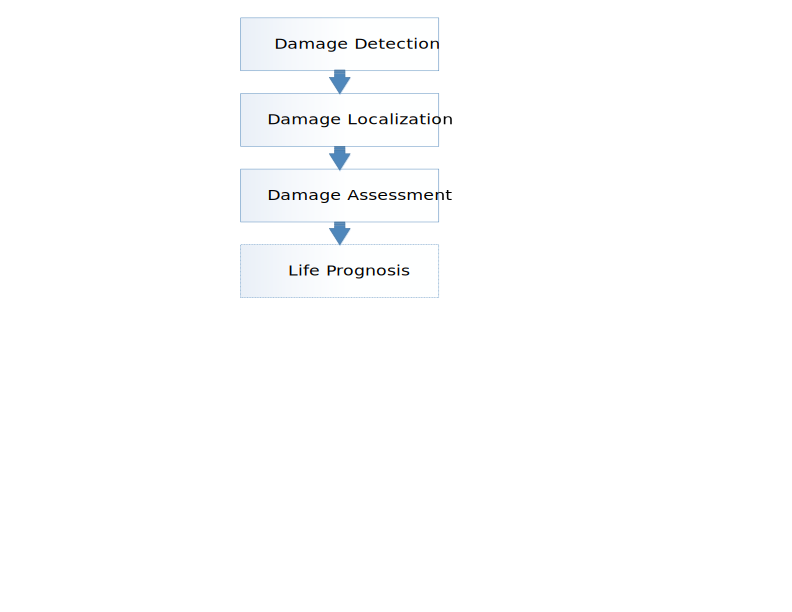
\includegraphics[width=0.7\textwidth]{fig1.1.png}
	\end{center}
	\caption{Five Main levels of SHM Techniques} 
	\label{fig:fig1.1}
\end{figure}

According to these levels, detection gives a qualitative explanation that the damage may exist, localization gives an indication about the probable position of the damage, assessment indicates the estimation of damage severity by giving information about the size and type of damage and at last, the estimation of residual structural life is provided at remaining life and smart structures (prognosis) stage. It also predicts possible failures or breakdowns. The first three levels (i.e. detection, localization, and assessment) are usually related to system identification, signal processing, and modelling aspects. The last two levels fall into statistical analysis, reliability, fatigue analysis, fracture mechanics, and design assessment fields. Many researchers have comprehensively investigated the last two levels but currently, there are no commercially available solutions.\cite{stepinski2013advanced,TibaduizaBurgos2020}. 


\section{SHM and Nondestructive Evaluation/Testing (NDE/T)}
%%%%%%%%%%%%%%%%%%%%%%%%%%%%%%%%%%%%%%%%%%%%%%%%%%
Damage detection/monitoring, NDT/E and SHM are usually mixed up as same things and may have the same meaning in many engineering areas. Health, damage, and monitoring of structures can be interpreted using different definitions. Generally, health is the ability to perform and maintain structural integrity all over the whole lifetime of the structure. However, monitoring is the process of assessment and prognosis, and damage is a material which is functional or structural failure.\cite{stepinski2013advanced}.

Typically, SHM is identified as online�global damage identification method in
structural systems. Whereas, NDE is usually performed as off-line in a local manner once the damage has been located or periodically, for improving the performance of a structure. However, it is not essential as NDE is also used as a monitoring tool for in situ structures such as rails and pressure vessels. NDE is primarily used for severity check and damage characterization when the damage location is already known.\cite{Farrar2007,Farrar2012}.

SHM involves integrating actuators and sensors, possibly smart materials, computational power and data transmission within a structure in order to detect, assess, localize, and predict damage. A typical SHM system is concerned with an online global damage identification in structures; SHM based systems are most often applied in civil engineering and aerospace. SHM systems employ NDT/E methods as tools, however, there are many differences in SHM and NDT/E operation principles\cite{stepinski2013advanced}. 

NDT techniques are often bounded to single point measurements. SHM methods allow for online monitoring of large structures and also can perform damage localization. With new sensors, SHM based methods are suitable for reliable continuous monitoring. For reliable damage detection, the SHM needs more state-of-the-art signal processing than classical NDT techniques \cite{stepinski2013advanced}.

The main difference between SHM and NDT techniques can be observed from the hardware architecture. In the case of a SHM system, actuators and sensors are integrated with or built into the structure, while there is no integration involved with the structure in the case of NDT. NDT is an external system with an independent set of actuators and sensors\cite{stepinski2013advanced}.

Most of the NDE techniques require component disassembly especially for the those components that are inaccessible which results in interruption of the daily operation of the structural systems leading to downtime which consequently results to an increase in operational costs. In an effort to improve on the integrity of structures, SHM technology has been introduced for the monitoring of civil, mechanical, and aerospace structures (To cite No.10 here, 'Damage detection of structural elements based on active sensing and machine learning approaches').  
Most of the NDT methods are often expensive, time-consuming, and labor-intensive, and they depend heavily on the skill and experience of the operator. NDT measurements are generall qualitative, there is no direct reliability of measurements to get verified. 
There is a need for proper experience and skilled judgment. Safety precautions are essential for most of the NDT methods. SHM is mainly
focused on condition-based maintenance. It is becoming more important nowadays
in various engineering fields such as mechanical, civil, and aerospace. NDT methods are basically localized in nature [56] whereas SHM deals in a broader perspective. NDT requires a prior knowledge of the location of damage whereas there is no such requirement in SHM. SHM is a better and modified version of NDT [57]. Table 8.1 shows the main differences between NDT and SHM. SHM is able to save costs and maintain a proper level of safety taking into consideration the working conditions [59]. SHM is used widely by the aerospace community, especially in a situation of aging of aircrafts [60]. NDT is slowly moving toward a more lasting attachment and continuous monitoring, and hence toward
SHM [62]. Smaller and cheaper sensors have been brought into the process of
changing from NDT to SHM [63]. In NDT there is also a requirement of external
probes [64]. Disassembling is done in SHM only when required, thus helping to
reduce costs as compared to NDT, which requires high cost for maintaining of the
system. Thus SHM due to its many advantages over NDT has a good future in the
engineering field.

\section{Advantages of SHM}
%%%%%%%%%%%%%%%%%%%%%%%%%%%%%%%%%%%%%%%%%%%%%%%%%%
text

\section{Different Types of SHM}
%%%%%%%%%%%%%%%%%%%%%%%%%%%%%%%%%%%%%%%%%%%%%%%%%%
text

\section{Major Components of SHM}
%%%%%%%%%%%%%%%%%%%%%%%%%%%%%%%%%%%%%%%%%%%%%%%%%%
text

\section{Types of Sensors used in SHM}
%%%%%%%%%%%%%%%%%%%%%%%%%%%%%%%%%%%%%%%%%%%%%%%%%%
text

\section{Guided Waves Based SHM}
%%%%%%%%%%%%%%%%%%%%%%%%%%%%%%%%%%%%%%%%%%%%%%%%%%
text

\section{SHM in Composite Structures}
%%%%%%%%%%%%%%%%%%%%%%%%%%%%%%%%%%%%%%%%%%%%%%%%%%
text

\section{Major Challenges in SHM}
%%%%%%%%%%%%%%%%%%%%%%%%%%%%%%%%%%%%%%%%%%%%%%%%%%
text

\section{Artificial Intelligence, Machine Learning and Deep Learning}
%%%%%%%%%%%%%%%%%%%%%%%%%%%%%%%%%%%%%%%%%%%%%%%%%%
text

\section{AI, ML and DL in SHM}
%%%%%%%%%%%%%%%%%%%%%%%%%%%%%%%%%%%%%%%%%%%%%%%%%%
text


%%%%%%%%%%%%%%%%%%%%%%%%%%%%%%%%%%%%%%%%%%%%%%%%%%
%\subsection{Description}
%%%%%%%%%%%%%%%%%%%%%%%%%%%%%%%%%%%%%%%%%%%%%%%%%%
%text
%%%%%%%%%%%%%%%%%%%%%%%%%%%%%%%%%%%%%%%%%%%%%%%%%%

%\begin{figure} [h!]
%	\begin{center}
		%\includegraphics[width=14cm]{Graphics/bc.jpg}
%	\end{center}
%	\caption{Figure caption.} 
%	\label{fig:bc}
%\end{figure}

%%%%%%%%%%%%%%%%%%%%%%%%%%%%%%%%%%%%%%%%%%%%%%%%%%

%\begin{table}[h]
%\centering
%	\caption{Table caption}
%	\begin{tabular}{cccc}
%		\hline
%	\textbf{a}	& \textbf{x} & \textbf{y} & \textbf{z} \\
%		\hline
%		-50 & -0.289 & -0.289 & -0.598\\ 
%		-40 & -0.248 & -0.248 & -0.512\\ 
%		\hline 
%	\end{tabular} 
%	\label{tab:xyz}
%\end{table}
%%%%%%%%%%%%%%%%%%%%%%%%%%%%%%%%%%%%%%%%%%%%%%%%%%

%The scheme of experimental setup is shown in Fig.~\ref{fig:bc}.  
%The values are collected in Tab.~\ref{tab:xyz}.


%The details are described in a book~\cite{udd2011fiber}. 

%Similar case was analysed\cite{Badrinarayanan2017a} by Hill et al.
%Additional information:
%\begin{itemize}
%\item fonts Times New Roman, 11pt
%\item keep figures separately in greyscale with resolution 600 dpi (publisher requirement)
%\item 20-30 pages
%\item Bibliography\cite references in the order of citations within the text
%\end{itemize}

\bibliography{report} % 
%bibliography data in report.bib
\bibliographystyle{abbrv}
% makes bibtex use spiebib.bst


%%%%%%%%%%%%%%%%%%%%%%%%%%%%%%%%%%%%%%%%%%%%%%%%%%
\end{document}
%%%%%%%%%%%%%%%%%%%%%%%%%%%%%%%%%%%%%%%%%%%%%%%%%%
